
\appendix

\section{Backup}


\begin{frame}{Experimental data in NNPDF4.0}
    \vspace*{-1em}
    \begin{columns}
        \column{0.48\linewidth}
            {\footnotesize
            \begin{itemize}
                \item 44 new datasets included
                \item 323 more data points in NNPDF4.0 \\ than in NNPDF3.1
                \item New data is mostly from the LHC RUN II
            \end{itemize}
            }
            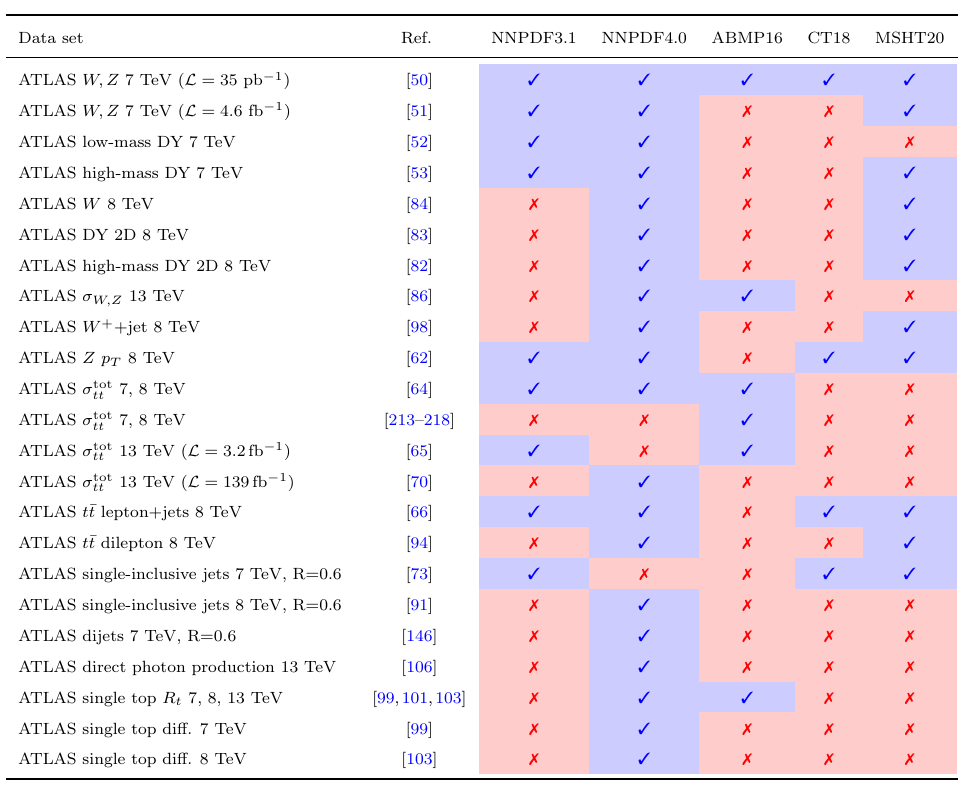
\includegraphics[width=0.9\textwidth]{atlas_data_table}
    
        \column{0.48\linewidth}
            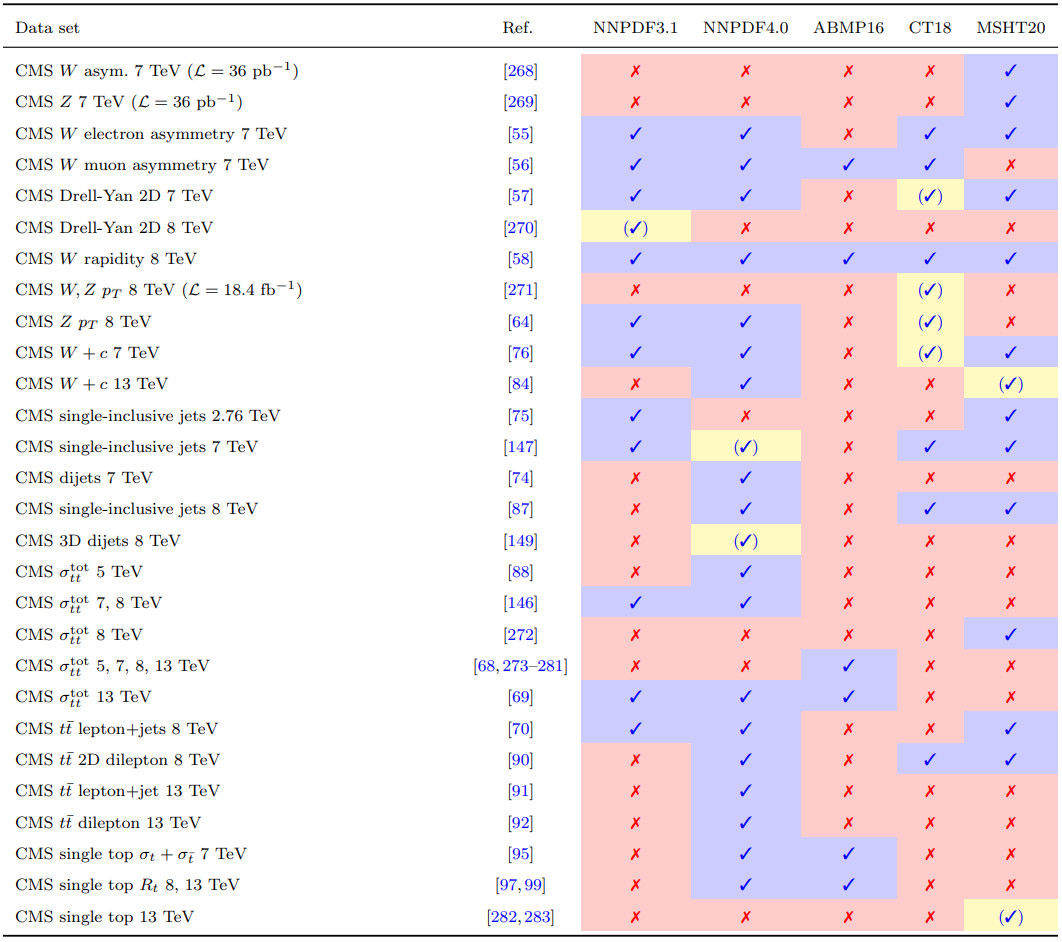
\includegraphics[width=0.9\textwidth]{cms_data_table} \\
            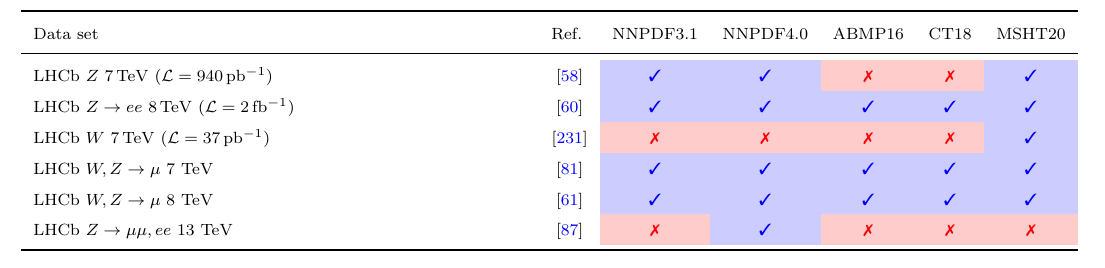
\includegraphics[width=0.9\textwidth]{lhcb_data_table}
    \end{columns}
\end{frame}


\begin{frame}{NNPDF4.0 model}{For more information see  \href{https://arxiv.org/pdf/1907.05075}{\color{blue} EPJ\,C79\,(2019)\,676}}
  \begin{figure}[t]
    \centering
    \resizebox{0.6\textwidth}{!}{%
      \begin{tikzpicture}[node distance = 1.0cm]\scriptsize
      % Input node
      \node (xinput) {$\{\mathrm{xgrid}_n\}$};
  
      % PDF basis
      \coordinate [right = 1.5cm of xinput] (NNghost) {};
      \node[fitted, above = 1.0cm of NNghost, minimum width=1.7cm, minimum height=0.7cm] (pdf) { Neural Net};
      \node[fitted, below = 1.0cm of NNghost, minimum width=1.7cm, minimum height=0.7cm] (preproc) { $x^{\alpha}$ $(1-x)^{\beta}$};
      \node[above = 0.6cm of pdf, minimum width=1.7cm, minimum height=0.3cm] (fform) 
      {\color{red} {\fontsize{10pt}{0}\selectfont $\mathrm{PDF}=Ax^\alpha(1-x)^\beta \mathrm{NN}(x,\log x)$} };
  
      % PDF production
      \node[operations, fill=violet!40, minimum width=1.2cm, minimum height=0.7cm, right = 1.5cm of NNghost]
          (fitbasis) {$\overline{\mathrm{PDF}}_n$};
      \node[operations, fill=violet!40, minimum width=1.2cm, minimum height=0.7cm, right = 0.6cm of fitbasis]
          (normalizer) {normalization};
  
      % PDFs 1 to n
      \node[right = 0.9cm of normalizer] (pdfdots) {\vdots};
      \node[above = 0.7cm of pdfdots] (pdf1) {PDF$_1$};
      \node[below = 0.7cm of pdfdots] (pdfn) {PDF$_n$};
  
      % Convolutions 1 to n
      \node[right = 0.2cm of pdf1] (conv1) {$\otimes$};
      \node[right = 0.2cm of pdfn] (convn) {$\otimes$};
      \node at ($(conv1)!0.5!(convn)$) (convdots) {$\otimes$};
  
      % FK Tables 1 to n
      \node[blue, right = 0.6cm of conv1] (f1) {$\hat{\sigma}_1$};
      \node[blue, right = 0.6cm of convn] (fn) {$\hat{\sigma}_n$};
      \node[blue] at ($(f1)!0.5!(fn)$) (fd) {\vdots};
      \draw[draw=blue, rounded corners] ($(f1.north west)+(-0.1, 0.2)$) rectangle ($(fn.south east)+(0.1,-0.2)$);
          \node[above = 0.6cm of f1] (theory) {Theory};
          \coordinate [above = 0.2cm of f1] (theoryarrow) {};
  
      % Observables
      \node[right = 0.5 cm of f1] (o1) {$\mathcal{O}_{1}$};
      \node[right = 0.5 cm of fn] (on) {$\mathcal{O}_{n}$};
      \node at ($(o1)!0.5!(on)$) (od) {\vdots};
      \node[above = 0.9cm of o1] (observables) {Observables};
      \coordinate [above = 0.2cm of o1] (observablearrow) {};
  
      % Tr/Vl split
      \node[operations, right = 0.5cm of od, minimum width = 1.2cm, text width=1cm, minimum height=0.7cm]
      (trvl) {Tr/Vl split};
      \coordinate [right = 1.0cm of trvl] (ending) {};
      \path let \p1 = (ending), \p2 = (pdf)
          in node at (\x1,\y2) [n3py, minimum width = 1.2cm, minimum height=0.7cm] (tr) {$\chi^{2}_\text{tr}$};
      \path let \p1 = (ending), \p2 = (preproc)
          in node at (\x1,\y2) [n3py, minimum width = 1.2cm, minimum height=0.7cm] (vl) {$\chi^{2}_\text{vl}$};
  
      % Arrows!
      \draw[myarrow] (xinput) -- (pdf);
      \draw[myarrow] (xinput) -- (preproc);
      \draw[myarrow] (pdf) -- (fitbasis);
      \draw[myarrow] (preproc) -- (fitbasis);
      \draw[myarrow] (fitbasis) -- (normalizer);
  
      \draw[myarrow] (pdf1) -- (conv1);
      \draw[myarrow] (pdfn) -- (convn);
      \draw[myarrow] (conv1) -- ($(f1.west)-(0.2,0.0)$) ;
      \draw[myarrow] (convn) -- ($(fn.west)-(0.2,0.0)$) ;
      \draw[myarrow] ($(f1.east)+(0.2,0.0)$) -- (o1);
      \draw[myarrow] ($(fn.east)+(0.2,0.0)$) -- (on);
  
      \draw[myarrow] (trvl) -- (tr);
      \draw[myarrow] (trvl) -- (vl);
      
      \draw[myarrow] (theory) -- (theoryarrow);
      \draw[myarrow] (observables) -- (observablearrow);
      
      % Braces
      \draw[decorate, decoration={brace}, thick] (pdfn.south west) -- (pdf1.north west);
      \draw[decorate, decoration={brace},thick] (o1.north east) -- (on.south east);
      \end{tikzpicture}
    }
  \end{figure}
  \textbf{Main changes:}
  \begin{itemize}
      \item \texttt{Python} codebase
          \begin{itemize}
              \item Easier and faster development
          \end{itemize}
      \item Freedom to use external libraries (default: \texttt{TensorFlow})
              \item Modularity $\Rightarrow$ ability to vary all aspects of the methodology
  \end{itemize}
\end{frame}



\begin{frame}{Performance benefit - time per replica}
  \begin{table}
     \renewcommand{\arraystretch}{1.50}
    \centering
    \begin{tabular}{c | c | c | c} \toprule
      & NNPDF3.1  & NNPDF4.0 (CPU) & NNPDF4.0  (GPU) \\
            \midrule
      Fit timing per replica    & 15.2 h        & 38 min        & 6.6 min \\ \hline
             Speed up factor    & 1        &  24      & 140 \\ \hline
      RAM use &  1.5 GB          &  6.1 GB                 & NA  \\ \bottomrule
    \end{tabular}
  \end{table}
  \vspace*{1em}
\end{frame}

\begin{frame}[t]{Hyperoptimization: the reward function}
    \begin{columns}[T]
        \begin{column}{0.48\textwidth}
            \vspace{\topsep}
            Choosing as the hyperoptimization target the $\chi^2$ of fitted data results in overfitting.
        \end{column}
        \begin{column}{0.48\textwidth}
            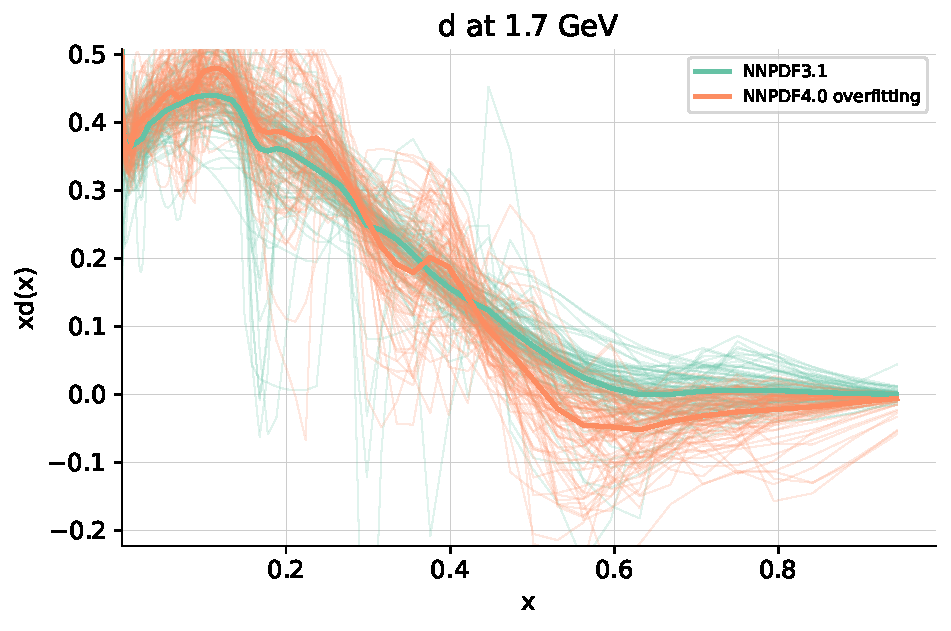
\includegraphics[width=0.9\textwidth]{overfit_nnpdf31}
        \end{column}
    \end{columns}
\end{frame}



\begin{frame}[t]{Hyperoptimization: the reward function}
    \begin{columns}[T]
        \begin{column}{0.48\textwidth}
            \vspace{\topsep}
            Choosing as the hyperoptimization target the $\chi^2$ of fitted data results in overfitting.\\
      \vspace*{2em}			
      We solve this using \textbf{k-fold cross-validation}:
      \begin{enumerate}
          \item Divide the data into $k$ {representative subsets}
          \item Fit $k-1$ sets and use $k$-th as test set
          \begin{itemize}
              \item[$\Rightarrow$] $k$ values of $\chi^2_\mathrm{test}$
          \end{itemize}
          \item Optimize the average $\chi^2_\mathrm{test}$ of the $k$ test sets
      \end{enumerate}
      \vspace*{0.5em}
      $\Rightarrow$ The hyperoptimization target is not based on data that entered the fit. 
        \end{column}
        \begin{column}{0.48\textwidth}
            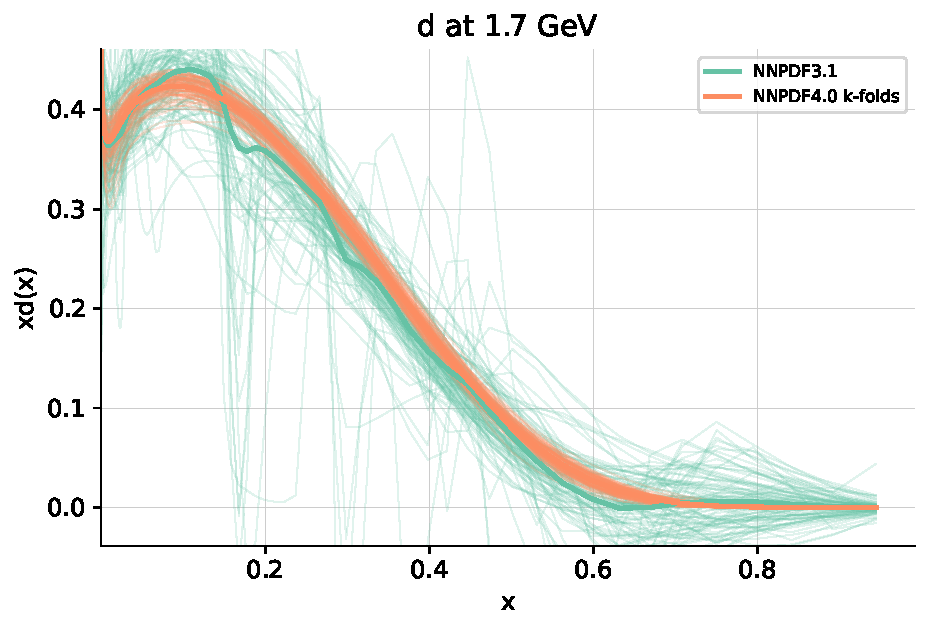
\includegraphics[width=0.9\textwidth]{best_model_vs_nnpdf31}
            \begin{itemize}
                \item No overfitting\\
          \vspace*{0.2em}
          \item Compared to NNPDF3.1:
          \begin{itemize}
              \item Increased stability
              \item Reduced uncertainties 
          \end{itemize}
      \end{itemize}
        \end{column}
    \end{columns}
\end{frame}

\begin{frame}{The (negligible) impact of datasets with tension}
    Excluding datasets with large $({\chi^{2}-1})/{\sigma_{\chi^{2}}}$ one at a time and combining the resulting PDFs following the conservative PDF4LHC15 prescription shows stability at the level of statistical fluctuations.
    \begin{columns}
        \begin{column}[T]{0.32\textwidth}
            \centering
            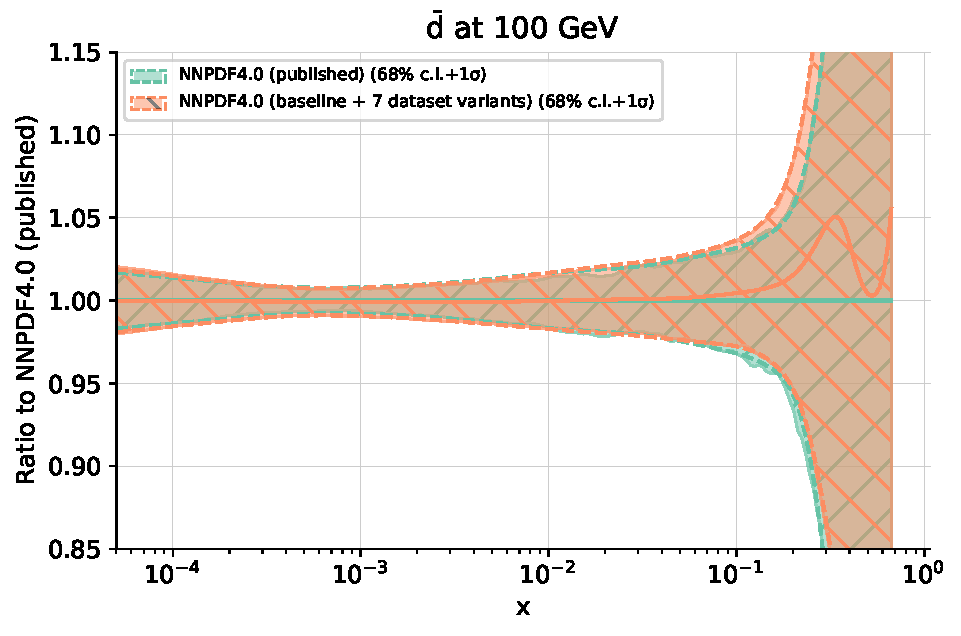
\includegraphics[width=0.9\textwidth]{env_bard.pdf}\\
            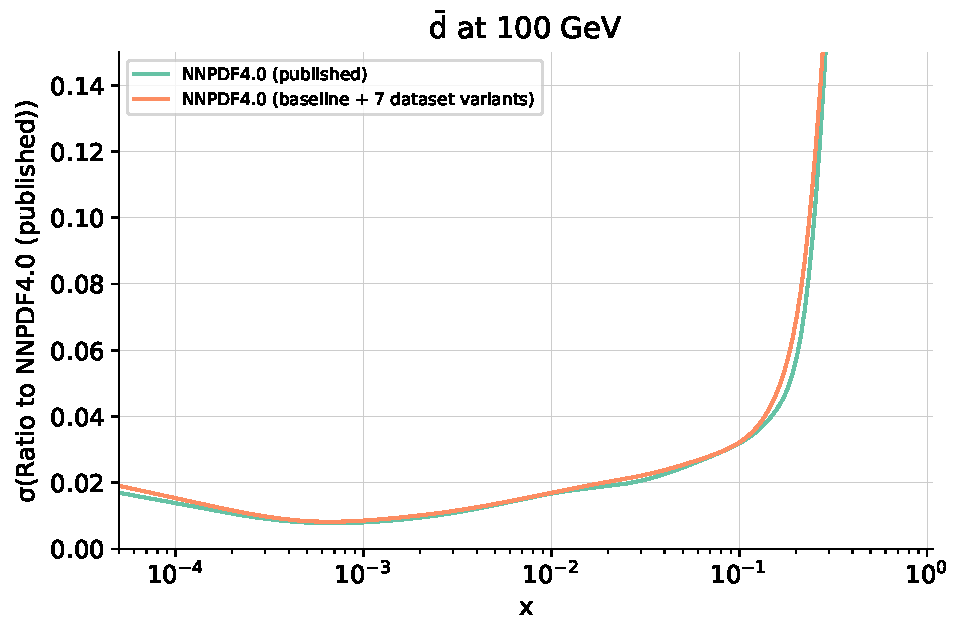
\includegraphics[width=0.9\textwidth]{envu_bard.pdf}
        \end{column}
        \begin{column}[T]{0.32\textwidth}
            \centering
            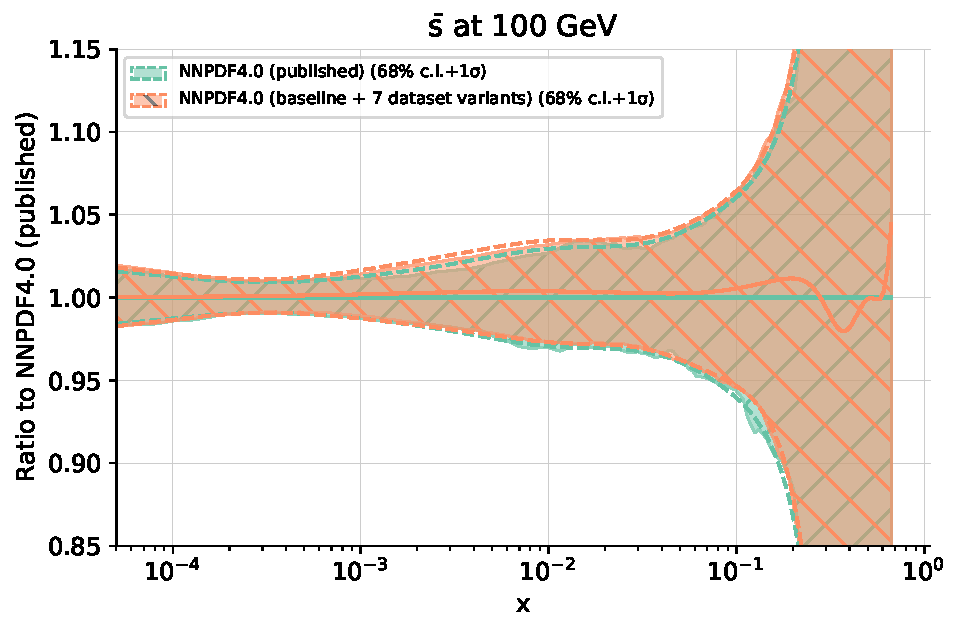
\includegraphics[width=0.9\textwidth]{env_bars.pdf}\\
            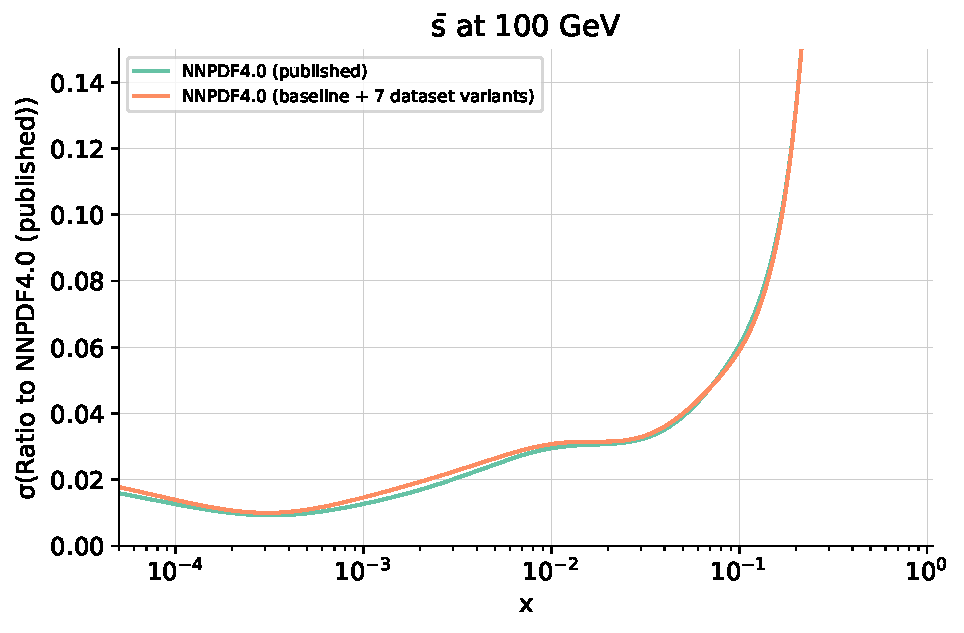
\includegraphics[width=0.9\textwidth]{envu_bars.pdf}
        \end{column}
        \begin{column}[T]{0.32\textwidth}
            \centering
            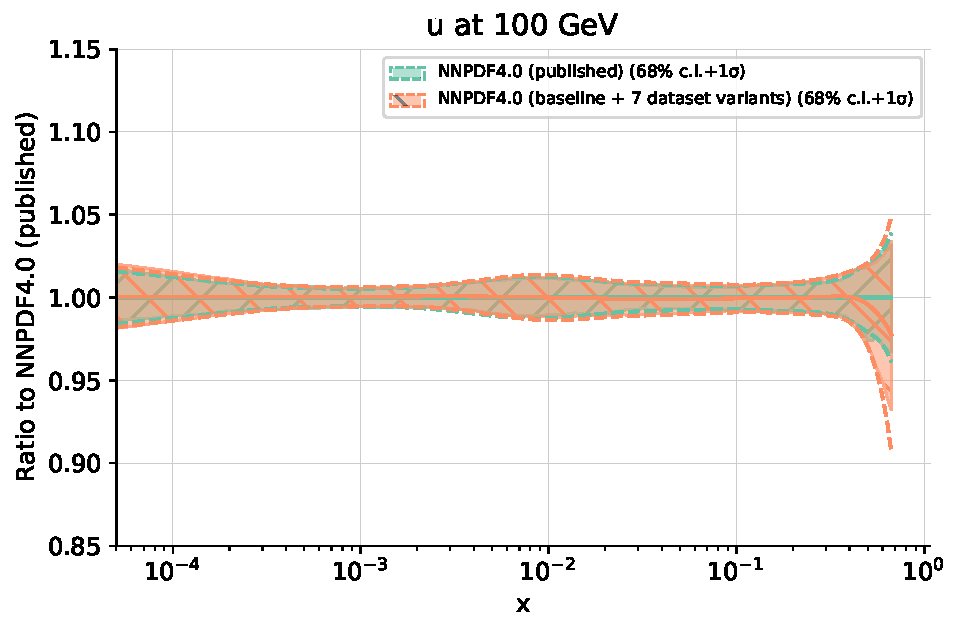
\includegraphics[width=0.9\textwidth]{env_u.pdf}\\
            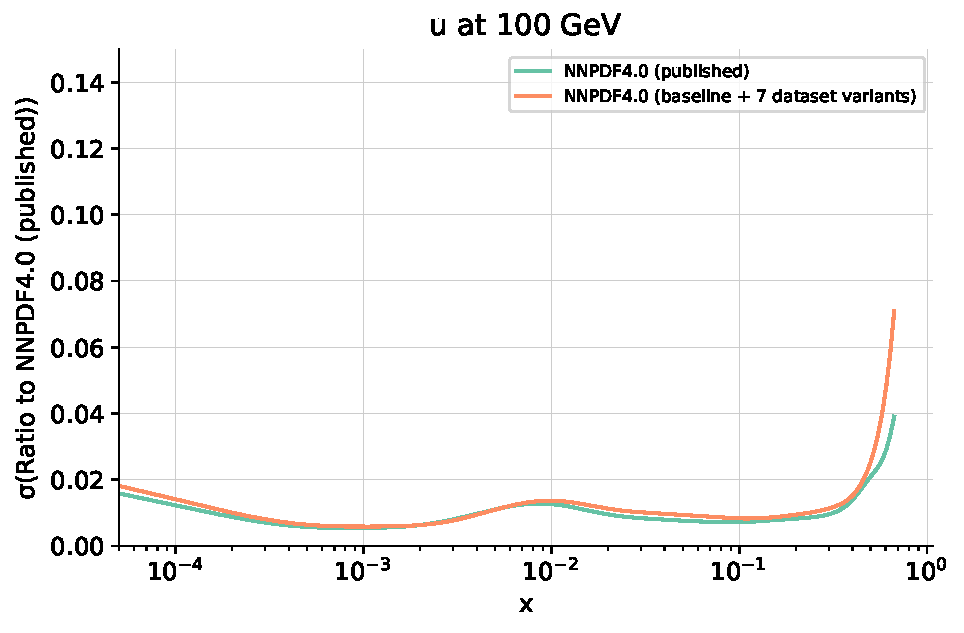
\includegraphics[width=0.9\textwidth]{envu_u.pdf}
        \end{column}
    \end{columns}
\end{frame}


\begin{frame}{Envelope of fits with different arametrization bases}
    Different strategies to parametrize the PDF flavour combinations lead to the same result
    \vspace*{-1em}
    \begin{columns}
        \begin{column}[T]{0.32\textwidth}
          \begin{center}
              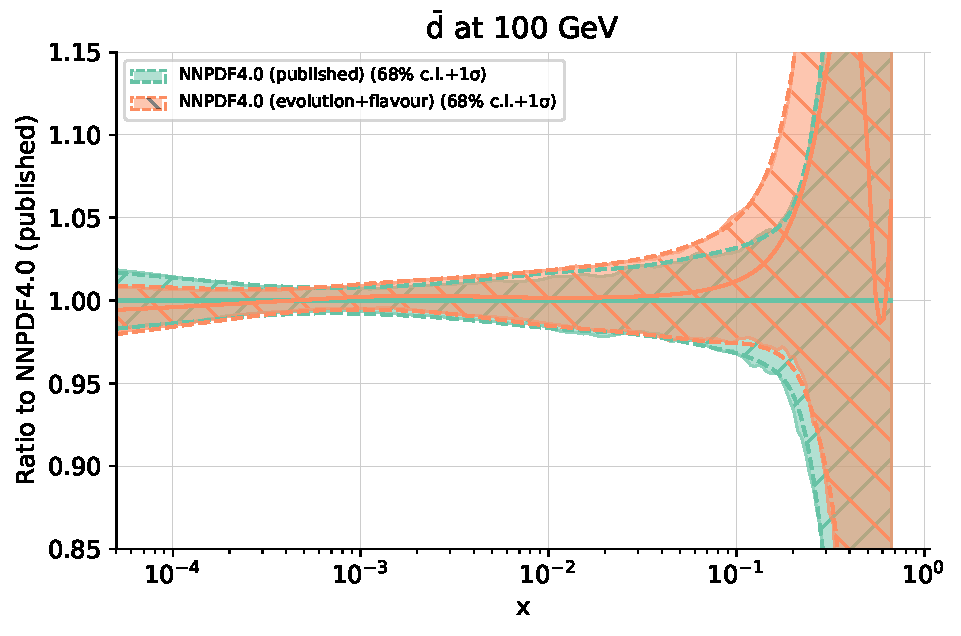
\includegraphics[width=0.95\textwidth]{efenv_bard.pdf} \\
              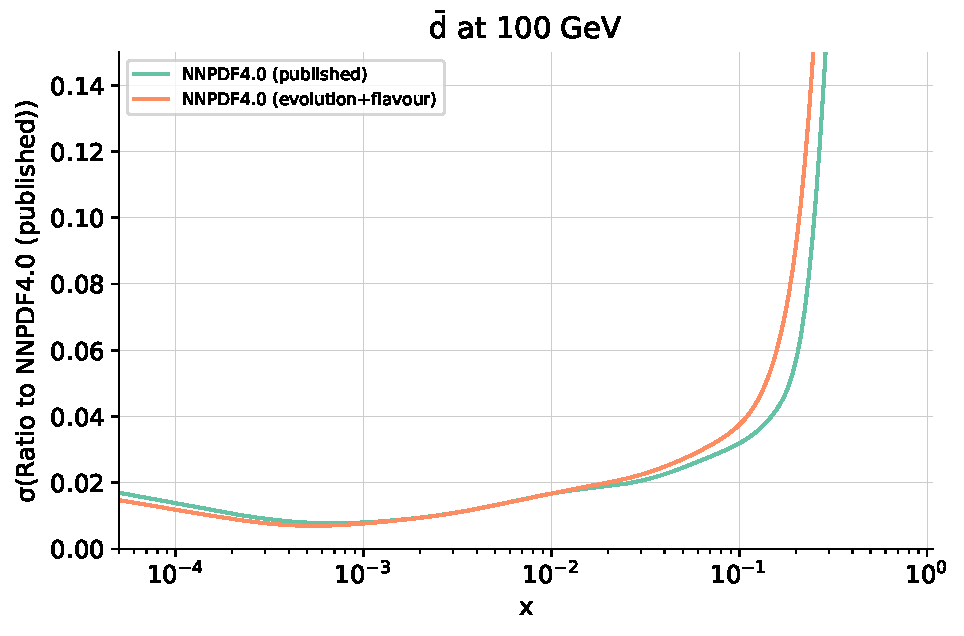
\includegraphics[width=0.95\textwidth]{efenvu_bard.pdf} 
          \end{center}
        \end{column}
        \begin{column}[t]{0.32\textwidth}
          \begin{center}
              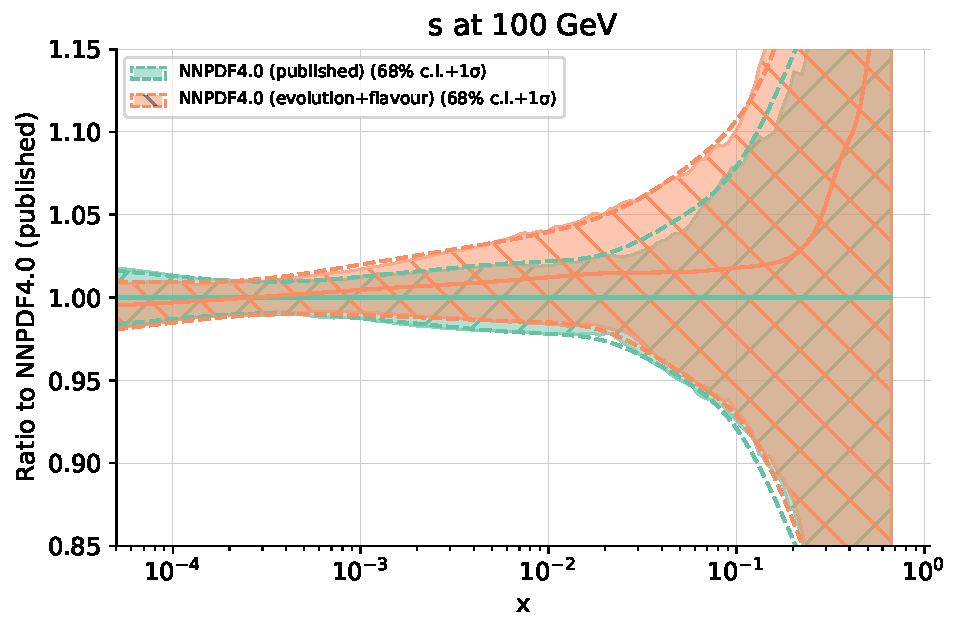
\includegraphics[width=0.95\textwidth]{efenv_s.pdf} \\
              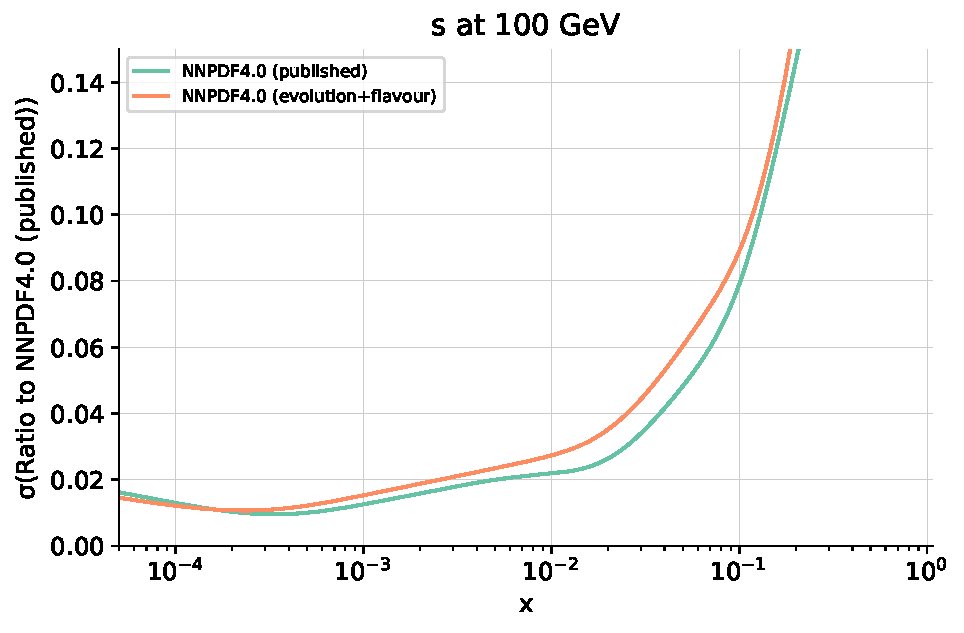
\includegraphics[width=0.95\textwidth]{efenvu_s.pdf} 
          \end{center}
        \end{column}
        \begin{column}[t]{0.32\textwidth}
            \begin{center}
                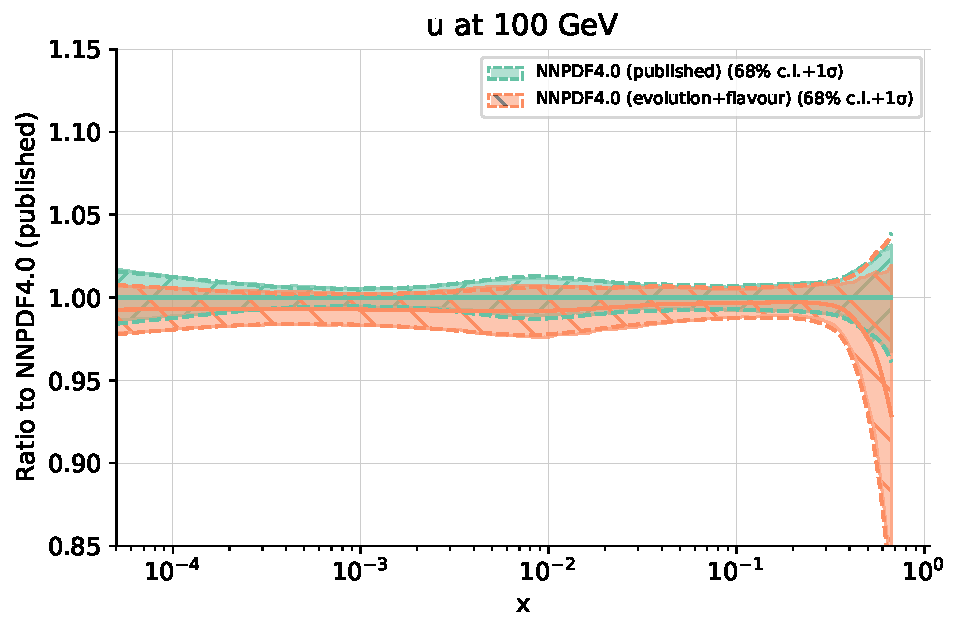
\includegraphics[width=0.95\textwidth]{efenv_u.pdf} \\
                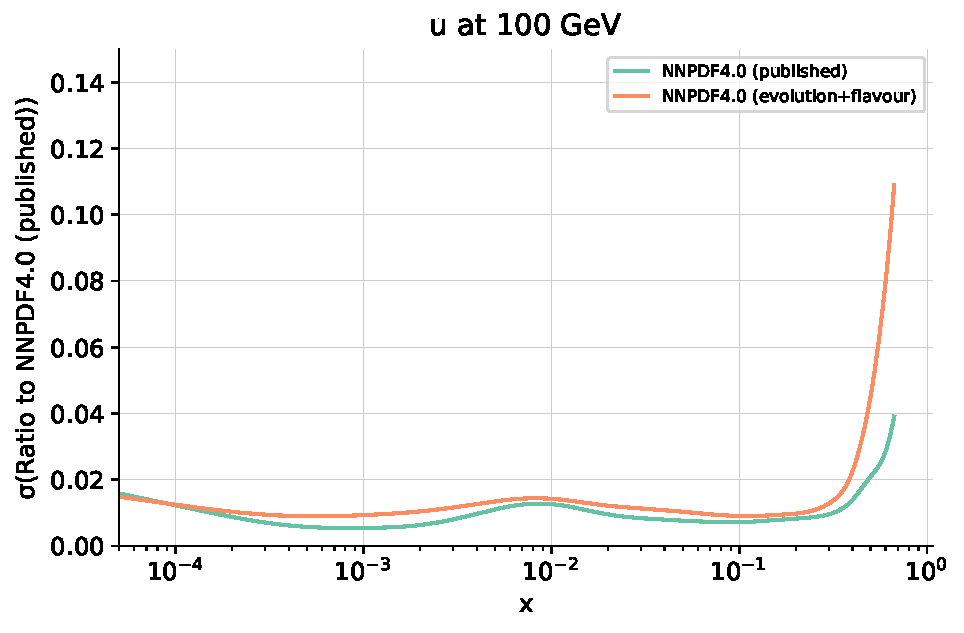
\includegraphics[width=0.95\textwidth]{efenvu_u.pdf} 
            \end{center}
          \end{column}
    \end{columns}
    % \begin{columns}
    %     \begin{column}{0.25\textwidth}
    %         \centering
    %         Evolution Basis:
    %         {\footnotesize
    %             \begin{fleqn}
    %                 \begin{align*}
    %                     \qquad x V\left(x, Q_{0}\right) &\propto \mathrm{NN}_{V}(x)\\
    %                     x T_{3}\left(x, Q_{0}\right) &\propto \mathrm{NN}_{T_{3}}(x)
    %                 \end{align*}
    %             \end{fleqn}
    %         }
    %     \end{column}
    %     \begin{column}{0.75\textwidth}
    %         \centering
    %         Flavour Basis:
    %         {\footnotesize
    %             \begin{fleqn}
    %                 \begin{align*}
    %                     \qquad x V\left(x, Q_{0}\right) &\propto\left(\mathrm{NN}_{u}(x)-\mathrm{NN}_{\bar{u}}(x)+\mathrm{NN}_{d}(x)-\mathrm{NN}_{\bar{d}}(x)+\mathrm{NN}_{s}(x)-\mathrm{NN}_{\bar{s}}(x)\right) \\
    %                     x T_{3}\left(x, Q_{0}\right) &\propto\left(\mathrm{NN}_{u}(x)+\mathrm{NN}_{\bar{u}}(x)-\mathrm{NN}_{d}(x)-\mathrm{NN}_{\bar{d}}(x)\right)
    %                 \end{align*}
    %             \end{fleqn}
    %         }
    %     \end{column}
    % \end{columns}
\end{frame}


\begin{frame}{Understanding the $\chi^2$ distribution}
    \begin{columns}
        \begin{column}[T]{0.48\textwidth}
            \centering
            Experimental $\chi^2$
            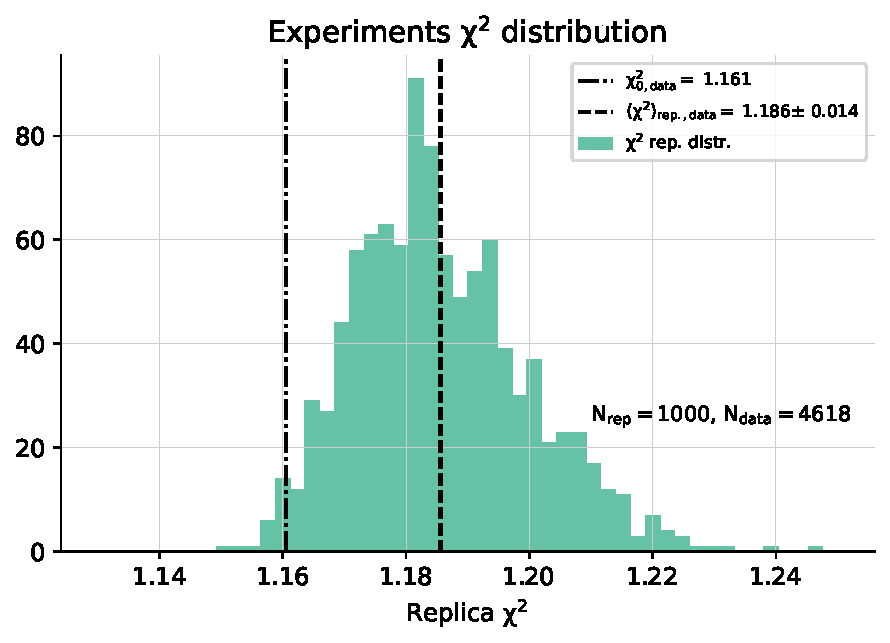
\includegraphics[width=\textwidth]{c2hist.pdf}
        \end{column}
        \begin{column}[T]{0.48\textwidth}
            \centering
            $t_0$ $\chi^2$
            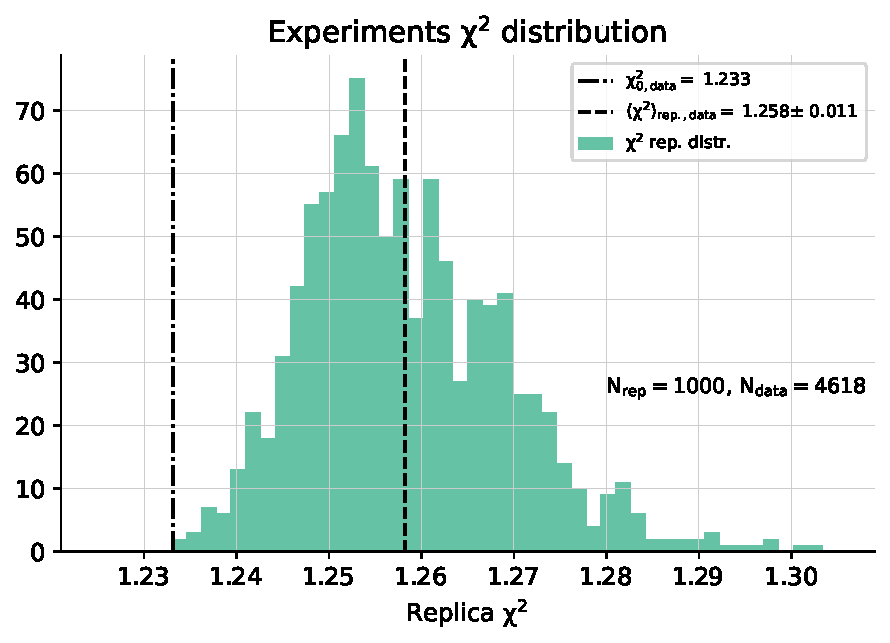
\includegraphics[width=\textwidth]{c2histt0.pdf}
        \end{column}
    \end{columns}
\end{frame}


\begin{frame}[t]{Impact of positivity on the PDFs}
    \begin{center}
        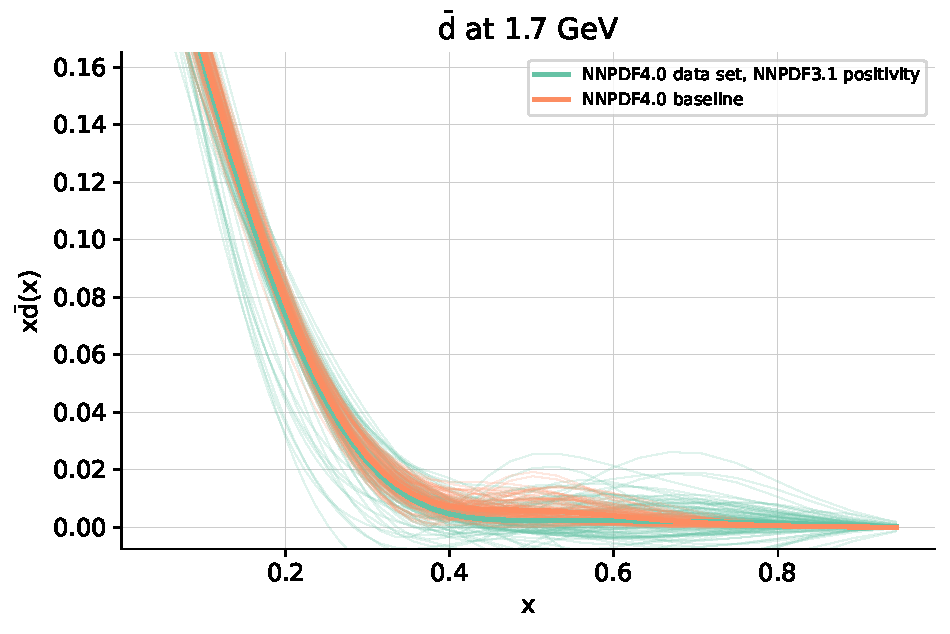
\includegraphics[width=0.6\textwidth]{dbpos.pdf}
    \end{center}
\end{frame}



\begin{frame}{More implications for phenomenology}
    \begin{columns}
        \begin{column}[T]{0.32\textwidth}
            \centering
            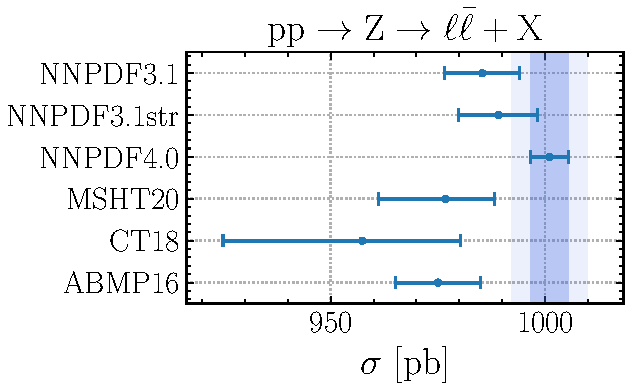
\includegraphics[width=\textwidth]{NNPDF_DY_14TEV_40_PHENO-integrated.pdf}
        \end{column}
        \begin{column}[T]{0.32\textwidth}
            \centering
            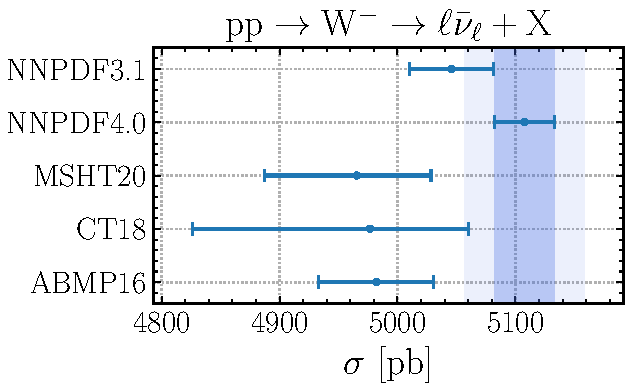
\includegraphics[width=\textwidth]{NNPDF_WM_14TEV_40_PHENO-integrated.pdf}\\
        \end{column}
        \begin{column}[T]{0.32\textwidth}
            \centering
            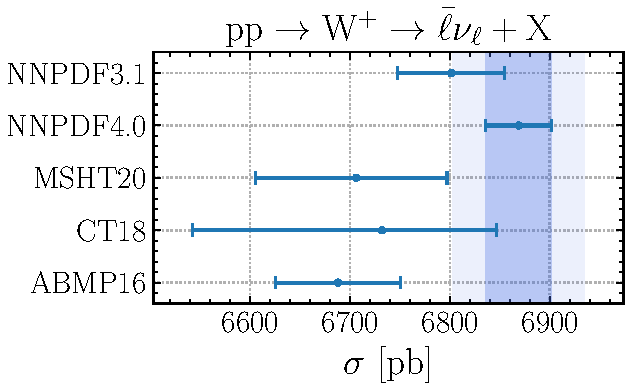
\includegraphics[width=\textwidth]{NNPDF_WP_14TEV_40_PHENO-integrated.pdf}
        \end{column}
    \end{columns}
\end{frame}

